\section{Lato Android}
Per quanto rigurda la fase di testing di quanto implementato per il client Android sono stati sfruttati principalmente due tool:
\begin{itemize}
	\item \textbf{Junit} per l'analisi dinamica del codice, con lo scopo quindi di verificare che il codice scritto funzioni in maniera coerente a quanto richiiesto e che vengano seguite le richieste descritte nei casi d'uso.
	\item \textbf{Espresso Junit} per l'analisi dell'interfaccia grafica costruita per la gestione delle varie richieste. Anche in questo caso si è fatto riferimento a quanto descritto dai casi d'uso riguardo alle view e al loro formato per osservare la correttezza di quanto implementato. 
\end{itemize}
\subsection{Espresso Junit}
Come detto, \textbf{Espresso Junit} è un tool attraverso il quale è possibile verificare le interazioni di un applicativo Android con l'utente. In questo caso quindi gli \textit{assert} verificano, ad esempio, che il fragment aperto sia quello corretto e che i campi dei vari componenti inseriti abbiano il valore desiderato.

Nell'ambito di questa iterazione, le componenti che sono state testate con questo applicativo sono quelle di:
\begin{enumerate}
	\item Login
	\item Registrazione manuale di un libro
	\item Ricerca di un libro
\end{enumerate}

Consideriamo, come esempio per la descrizione, il test relativo alla ricerca di un libro all'interno della rete di Book Crossing. Il test si compone nel seguente modo:
\begin{lstlisting}
@Test
public void searchBookTestOK(){
	Globals.isLoggedIn = true;
	Globals.usernameLoggedIn = "A";
	onView(withId(R.id.navigation)).check(matches(isDisplayed()));
	onView(withId(R.id.book_search)).perform(click());
	onView(withId(R.id.book_search)).check(matches(isDisplayed()));
	
	ViewInteraction checkTitle = onView(withId(R.id.title_search));
	ViewInteraction checkAuthor = onView(withId(R.id.author_search));
	ViewInteraction checkBtnSearch = onView(withId(R.id.search_button));
	
	checkTitle.check(matches(isDisplayed()));
	checkAuthor.check(matches(isDisplayed()));
	checkAuthor.check(matches(isDisplayed()));
	
	checkTitle.perform(setTextInTextView(""));
	checkAuthor.perform(setTextInTextView(""));
	
	checkTitle.perform(setTextInTextView("questa storia"));
	checkBtnSearch.perform(click());
	
	onView(withId(R.id.books_found)).check(matches(isDisplayed()));
	onData(anything()).inAdapterView(withId(R.id.books_found)).
	atPosition(0).perform(click());
	onView(withText(containsString("BOOKABLE"))).
	inRoot(withDecorView(not(mainActivityActivityTestRule.getActivity().getWindow().
	getDecorView()))).check(matches(isDisplayed()));
\end{lstlisting}

	\begin{figure}[h!]
	\centering
	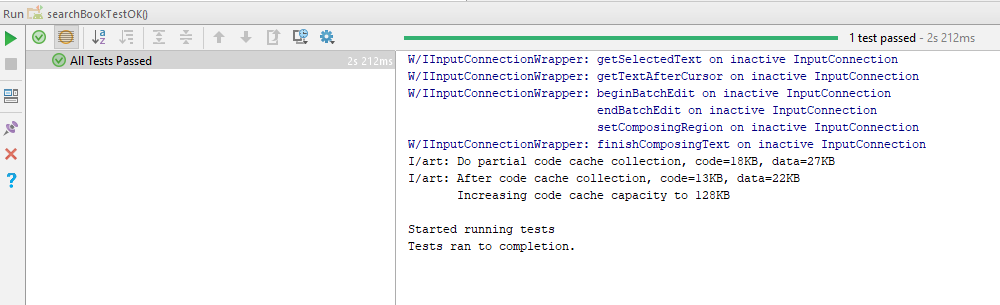
\includegraphics[width=0.8\textwidth]{Immagini/Test/Espresso.png}
	\caption{Espresso test}
	\label{fig:espresso}
\end{figure}
Questo caso di test verifica che la ricerca di un libro venga svolta in maniera corretta, garantendo la visualizzazione dei corretti \textit{fragment} e dei \textit{Toast} formattati in maniera corretta. L'esito di questo caso di test eseguito attraverso il tool \textbf{Espresso Junit} fornito da Android Studio può essere riassunto dalla figura \ref{fig:espresso}.
La medesima procedura è stata implementata per le altre componenti descritte precedentemente; il fatto di utilizzare questo tool consente di svolgere anche un'analisi dinamica del codice, dal momento che se ci fosse un errore, la successione grafica subirebbe un crash, mostrando un segnale di errore e facendo fallire il caso di test previsto.

\section{Lato Server}
	\subsection{Analisi Dinamica}
		\subsubsection{JUNIT Test}
		In questa sezione viene presentato un esempio di analisi dinamica del codice per quanto riguarda il lato server. Come esempio da riportare nella documentazione si è scelto di valutare il caso di test relativo alla fase di login, sia nel caso in cui l'esito sia positivo sia in caso in cui l'esito sia negativo.
		\begin{lstlisting}
		@Test
		public void logintTest() {
		
		Profile u = new Profile();
		u.setUsername("A");
		u.setPassword("6b86b273ff34fce19d6b804eff5a3f5747ada4eaa22f1d49c01e52ddb7875b4b");
		assertTrue(LoginStatus.SUCCESS == u.login());
		
		u.setPassword("1");
		assertFalse(LoginStatus.SUCCESS == ProfileData.getInstance().login(u));
		assertTrue(LoginStatus.WRONG_PWD == ProfileData.getInstance().login(u));
		
		u.setUsername("paperino");
		assertTrue(LoginStatus.WRONG_USERNAME == ProfileData.getInstance().login(u));
		}
		
		@Test
		public void existLogin() {
		Profile u = new Profile();
		u.setUsername("A");
		
		assertTrue(Profile.existUser(u.getUsername()));
		
		u.setUsername("ZX");
		assertFalse(Profile.existUser(u.getUsername()));
		}
		\end{lstlisting}
		\begin{figure}[h!]
			\centering
			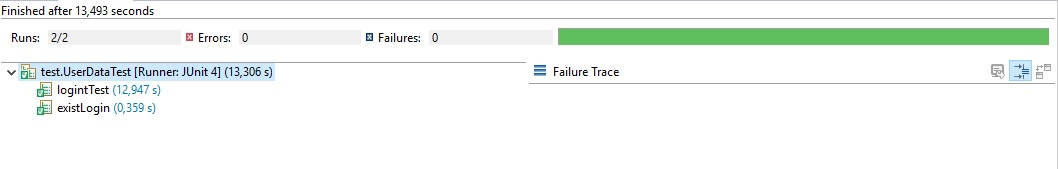
\includegraphics[width=\textwidth]{Immagini/Test/Junit_login.jpg}
			\caption{Junit test}
			\label{fig:Junit_login}
		\end{figure}
		L'esito è indicato dalla figura \ref{fig:Junit_login}, la quale evidenzia il fatto che inserendo username e password corretti, il login ha un esito successivo, al contrario si verifica che con delle credenziali sbagliate si verifica un errore.
		
		
	\subsection{Analisi Statica}
		\begin{figure}[h!]
			\centering
			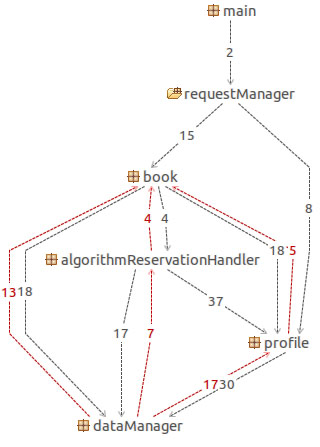
\includegraphics[width=0.3\textwidth]{Immagini/analisi_statica_package.jpg}
			\caption{Analisi statica del codice}
			\label{fig:analisiStatica}
		\end{figure}
		
		
		Nel seguente piano sono rappresentate le metriche di:
		\begin{itemize}
			\item Abstractness: misura quanto facilmente il sistema può essere espanso;
			\item Instability: tentativo di misurare la facilità di cambiamento. 
		\end{itemize}
\newpage
	\begin{figure}[h!]
		\centering
		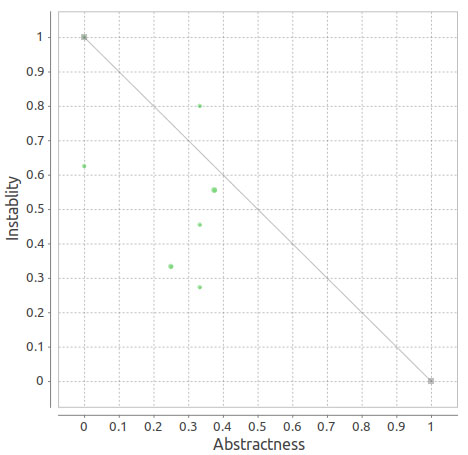
\includegraphics[width=0.3\textwidth]{Immagini/analisi_statica_grafico1.jpg}
		\caption{analisi statica grafico}
		\label{fig:analisiStaticaGrafico}
	\end{figure}		
I packages vicino al punto (0,0) sono rigidi mentre i packages vicino a (1,1) sono totalmente astratti e quindi inutili, idealmente vorremmo trovarci sulla linea rappresentata.
	
	
	
	
	
	
	
